\documentclass[a4paper]{article}

\usepackage[utf8]{inputenc}
\usepackage[T1]{fontenc}
\usepackage[spanish]{babel}
\usepackage[margin={20mm,25mm}]{geometry}

\usepackage{ifthen}
\usepackage{mathtools}
\usepackage{xcolor}
\usepackage{booktabs}
\usepackage{circuitikz}
\usepackage{fancyhdr}
\usepackage{parskip}
\usepackage{hyperref}
\usepackage{graphicx}

% --------------------
% DATOS DEL INFORME
\newcommand{\numeroTarea}   {2}                 % <-- Reemplazar X con el número de la tarea
\newcommand{\numeroGrupo}   {38}                 % <-- Reemplazar N con el número de su grupo
\newcommand{\nombrePrimero} {Diego Acevedo}    % <-- Reemplazar con el nombre del primer integrante
\newcommand{\rolPrimero}    {202023528-7}        % <-- Reemplazar con el rol del primer integrante
\newcommand{\nombreSegundo} {Diego Paz}    % <-- Reemplazar con el nombre del segundo integrante
\newcommand{\rolSegundo}    {202004502-k}        % <-- Reemplazar con el rol del segundo integrante
% --------------------

% --------------------
% NO MODIFICAR ESTA PARTE
\title{Informe Tarea \numeroTarea \\ \large
    \ifthenelse{\equal{\numeroTarea}{1}}{Circuito Combinacional}{}
    \ifthenelse{\equal{\numeroTarea}{2}}{Circuito Secuencial}{}
    \ifthenelse{\equal{\numeroTarea}{3}}{Lenguajes de Descripción de Hardware}{}
    \ifthenelse{\equal{\numeroTarea}{4}}{ARM Assembly}{}
    \ifthenelse{\equal{\numeroTarea}{X}}{Tema de la tarea}{}
}
\author{\textbf{Grupo \numeroGrupo} \\ \begin{tabular}{r @{\quad} l}
    \nombrePrimero & \rolPrimero \\
    \nombreSegundo & \rolSegundo
\end{tabular}}
\date{\today}

\setlength{\parindent}{15pt}
\addto\captionsspanish{\renewcommand{\tablename}{Tabla}}
% --------------------

\begin{document}

\begin{titlepage}
    \maketitle
    \thispagestyle{empty}
    
    \begin{abstract}
        Se nos pide crear un circuito secuencial en base al circuito combinacional que creamos para la tarea pasada, para esto se nos pide utilizar 15 registros de 6bits, en conjunto con un contador simple que nos indicase la cantidad de carga de la batería. Para esto fue necesario implementar distintos tipos de circuitos que son los bloques base para crear los registros, estos son los SR Latch, los D Latch y los D Flip Flop, una vez creados estos, pudimos crear los registros y a partir de eso, modificar el circuito original y crear el circuito secuencial que se nos encargó. Una vez terminado el circuito, pudimos testearlo con los casos de prueba entregados por los ayudantes para poder corroborar el buen y adecuado funcionamiento de nuestro circuito secuencial y poder realizar este informe de manera correcta.
    \end{abstract}
    
    \vfill
    \tableofcontents
\end{titlepage}

\section{Desarrollo de la tarea}
Para esta tarea se nos pide que, utilizando el circuito del la tarea anterior, creemos un circuito secuencial que pueda iterar en registros.

Partimos la tarea creando los componentes esenciales para la construccion de los registros, necesarios para realizar esta tarea:

\begin{figure}[!htbp]
    \centering
    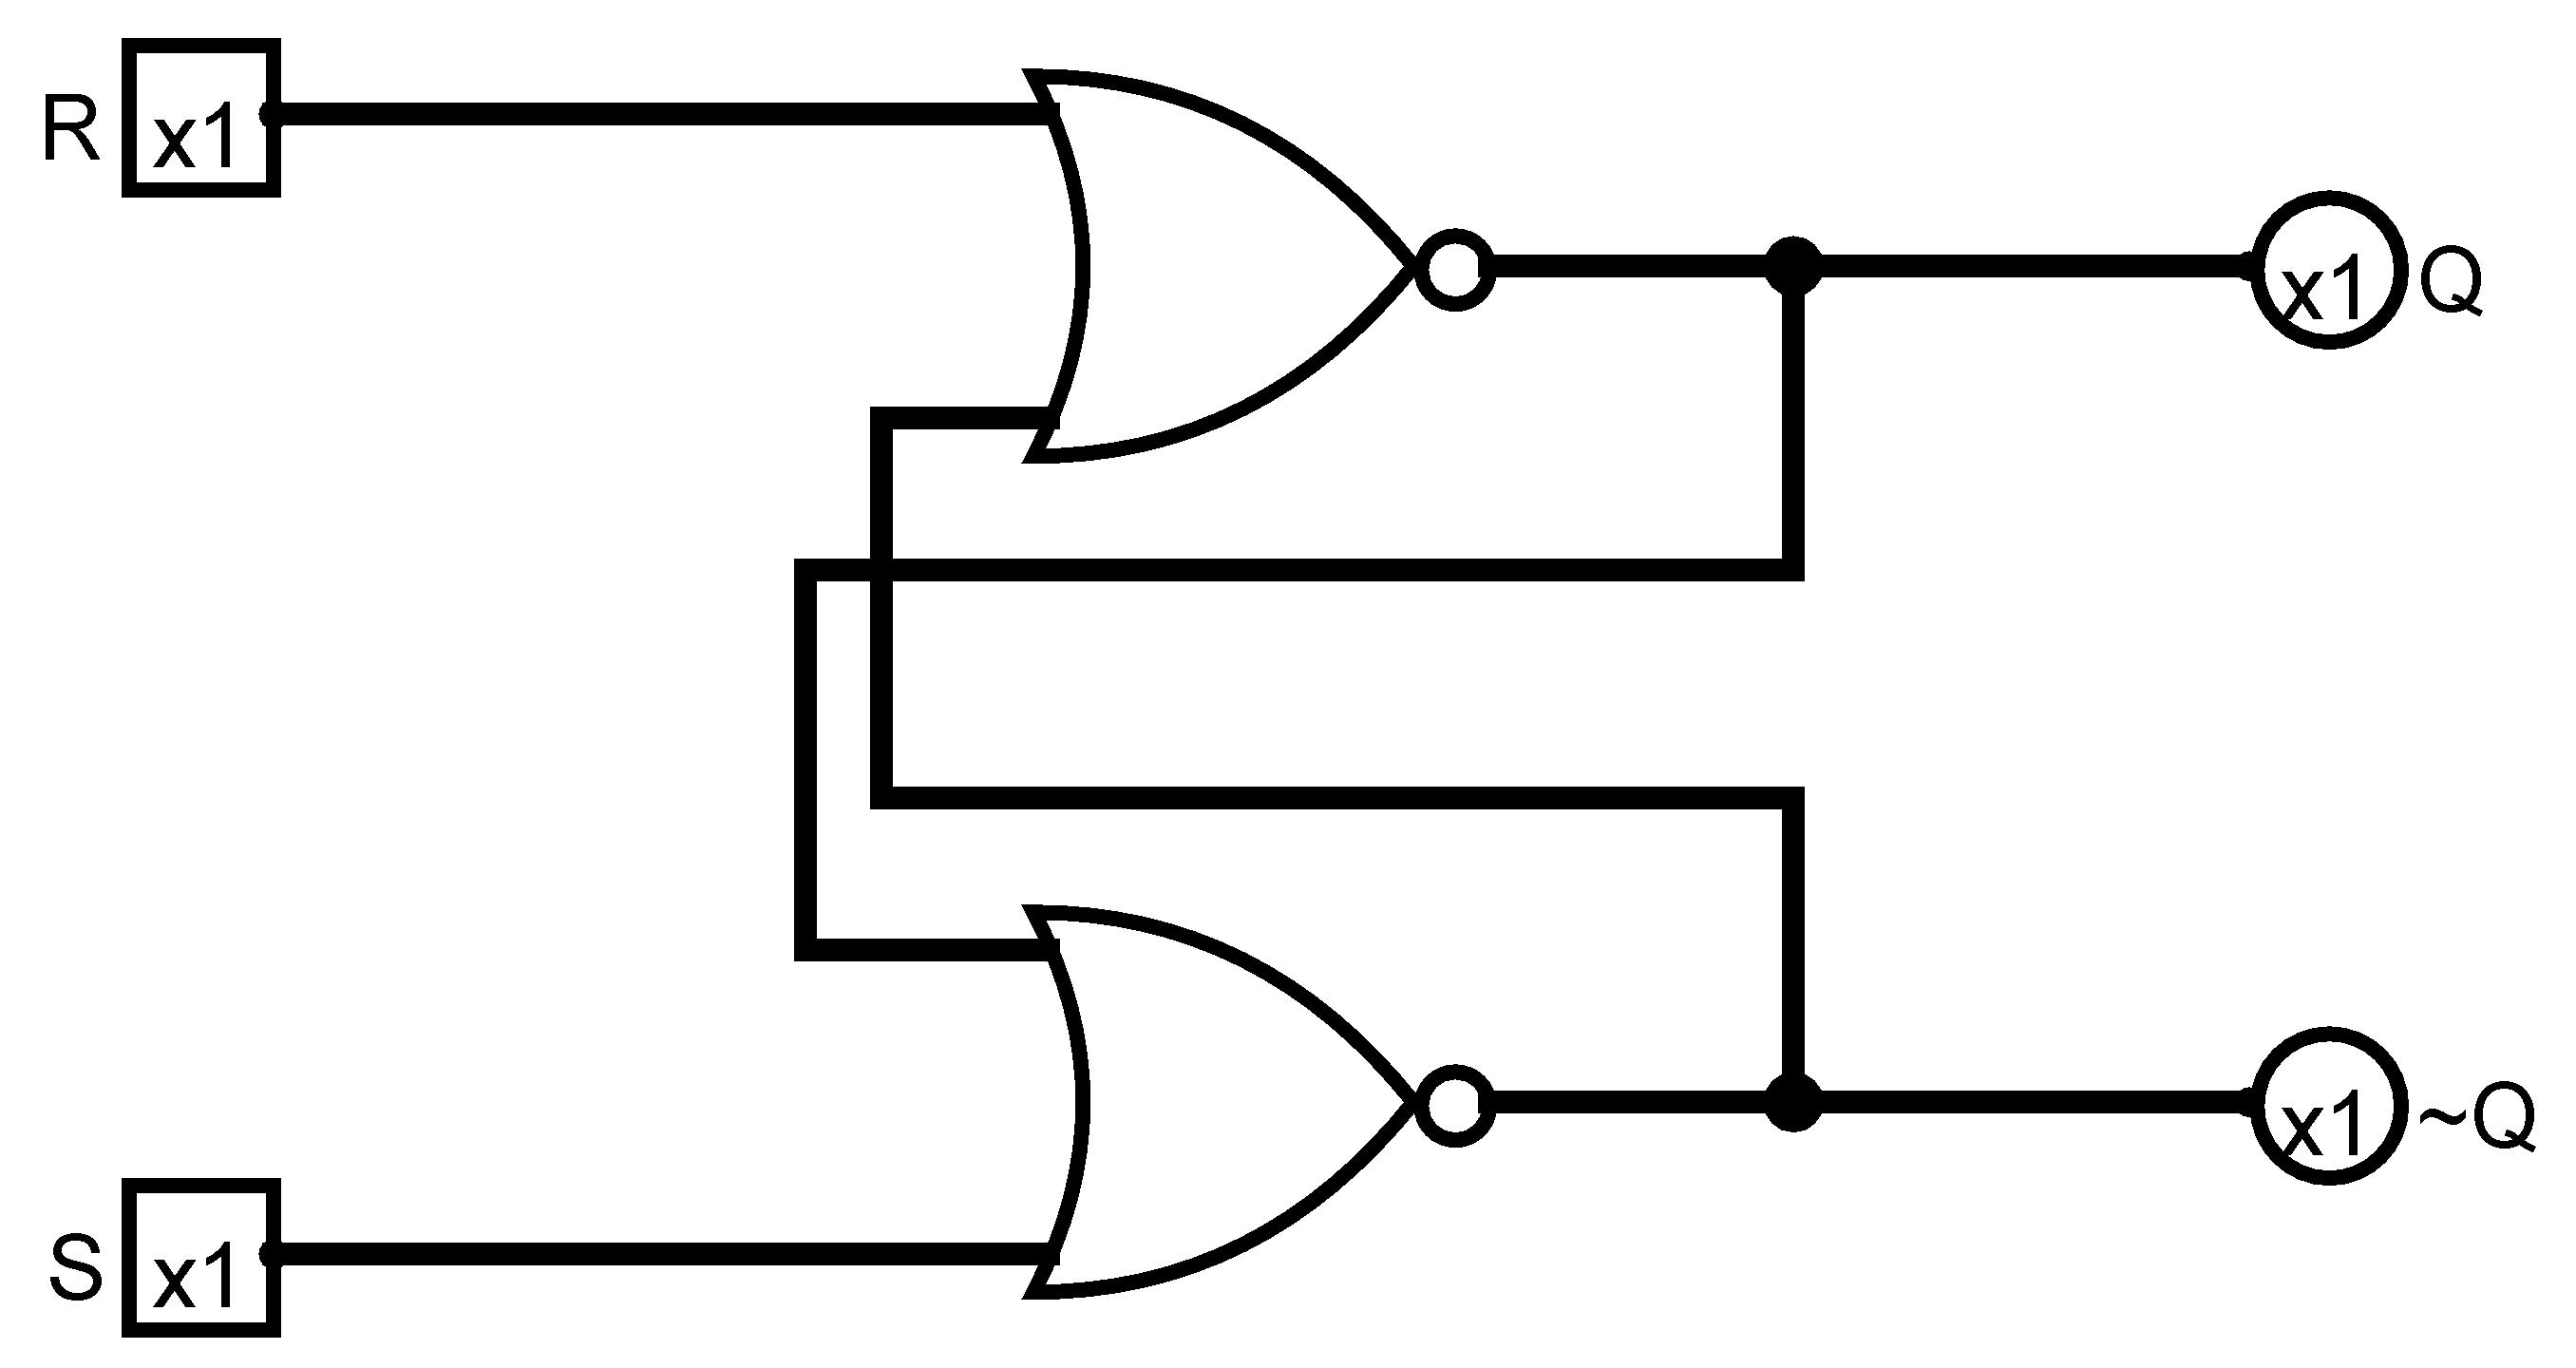
\includegraphics[width=0.5\textwidth]{SR Latch.jpg}
    \caption{Circuito digital del SR Latch.}
    \label{fig:SRLatch}
\end{figure}

El SR Latch se compone de 2 entradas de 1 bit, 2 puertas NOR y 2 salidas de 1 bit, la gracia de este circuito, es que al estar las 2 entradas en 0, las salidas se mantienen  en el ultimo estado conocido.

Utilizando el SR Latch, pasamos a crear el siguiente bloque necesario para crear los registros:

\begin{figure}[!htbp]
    \centering
    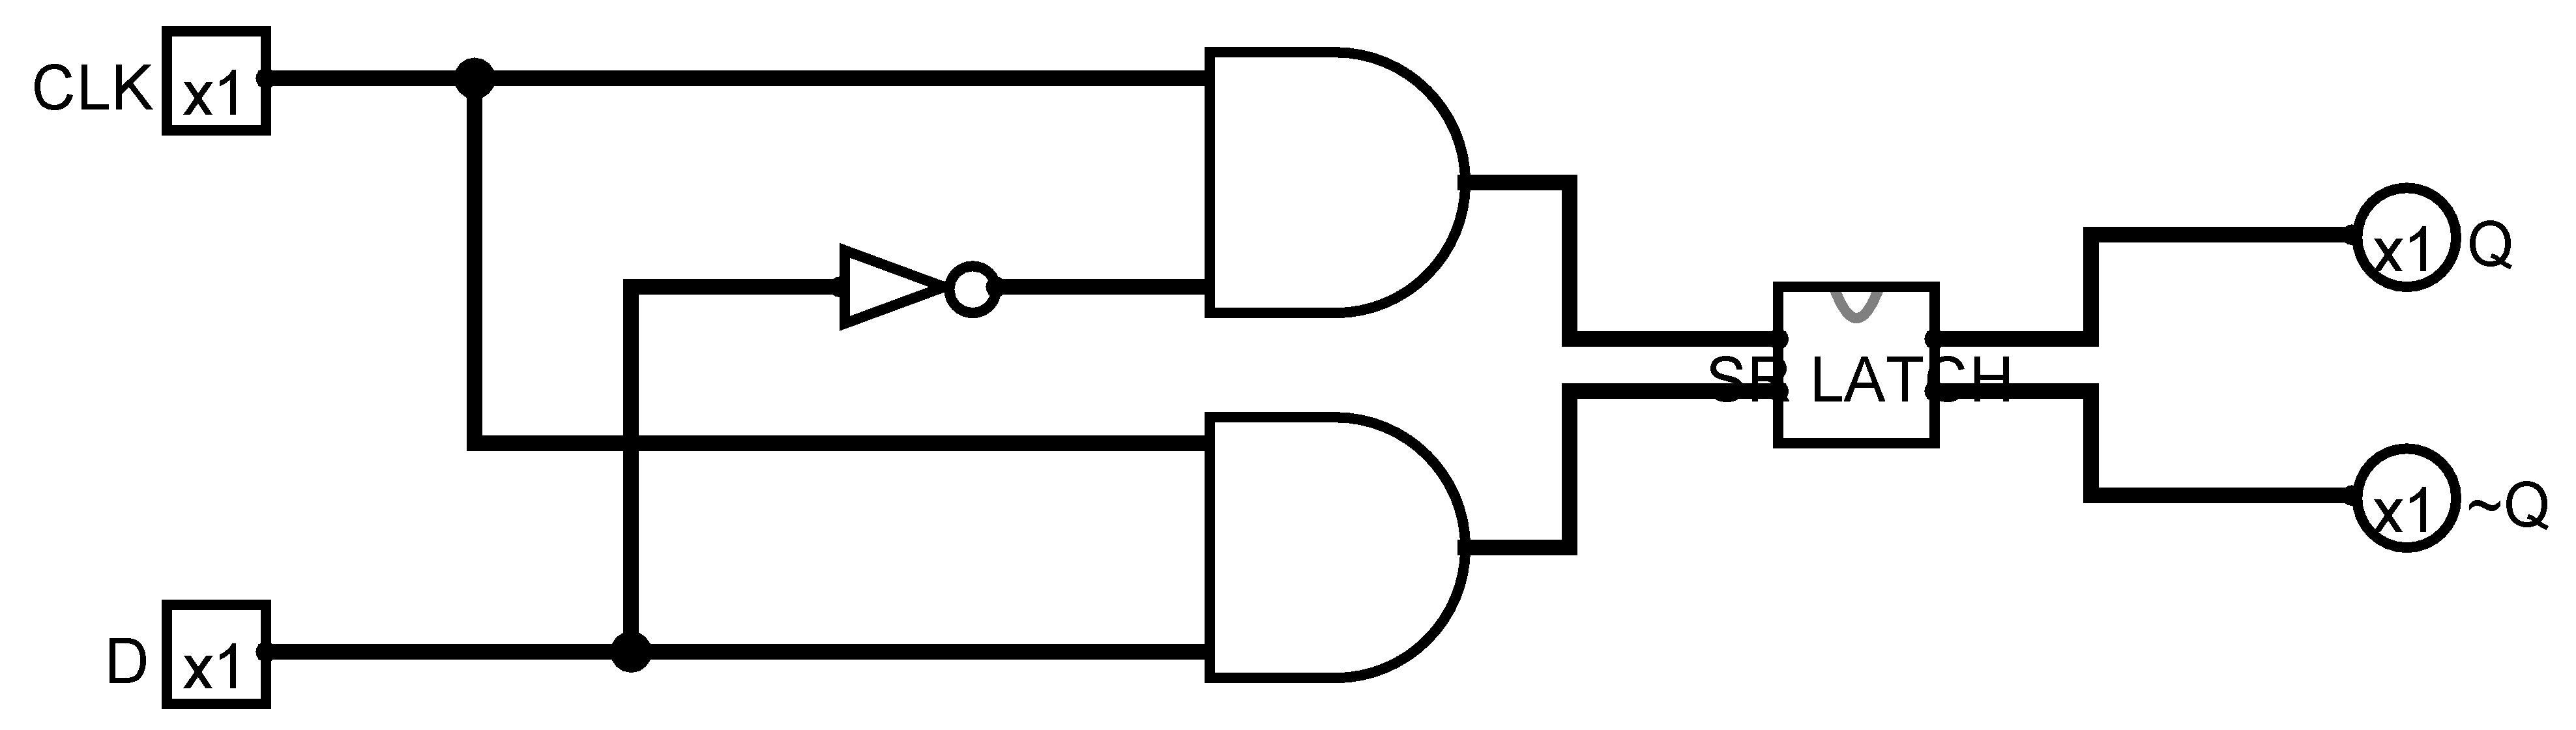
\includegraphics[width=0.6\textwidth]{D Latch.jpg}
    \caption{Circuito digital del D Latch.}
    \label{fig:DLatch}
\end{figure}

El D Latch es una adaptacion del SR Latch que resuelve los problemas de cuando y como cambia de estado al agregarse un \textit{Clock}.

Con el D Latch pasamos a crear otro bloque más:

\begin{figure}[!htbp]
    \centering
    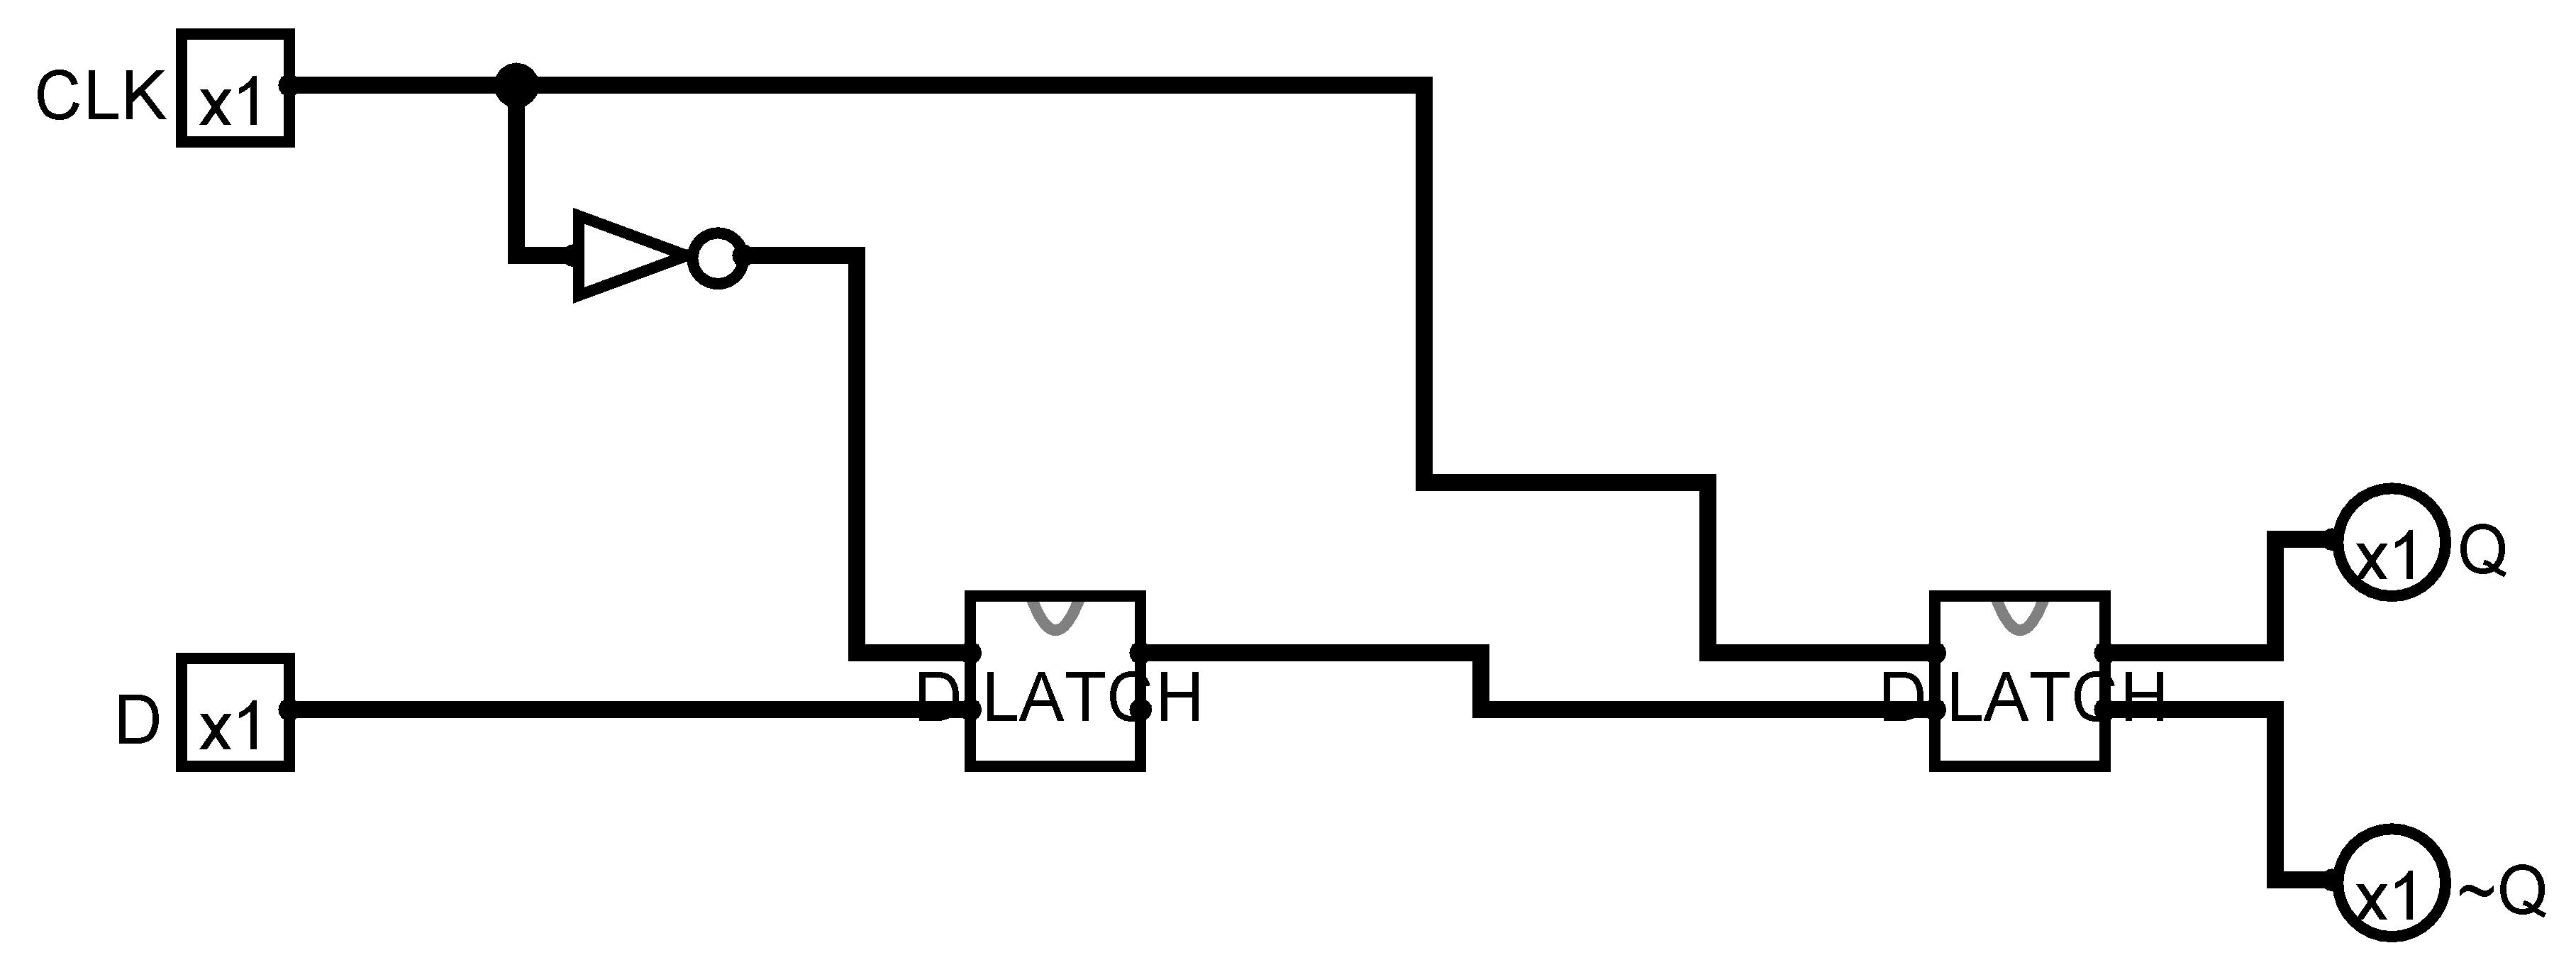
\includegraphics[width=0.6\textwidth]{D Flip Flop.jpg}
    \caption{Circuito digital del D Flip Flop.}
    \label{fig:DFlipFlop}
\end{figure}

El D Flip Flop está compuesto por 2 D Latch, y con un solo \textit{Clock}, controla cuando el valor de D se copia a Q.

Ya con este ultimo bloque, podemos crear los registros:

\newpage

\begin{figure}[!htbp]
    \centering
    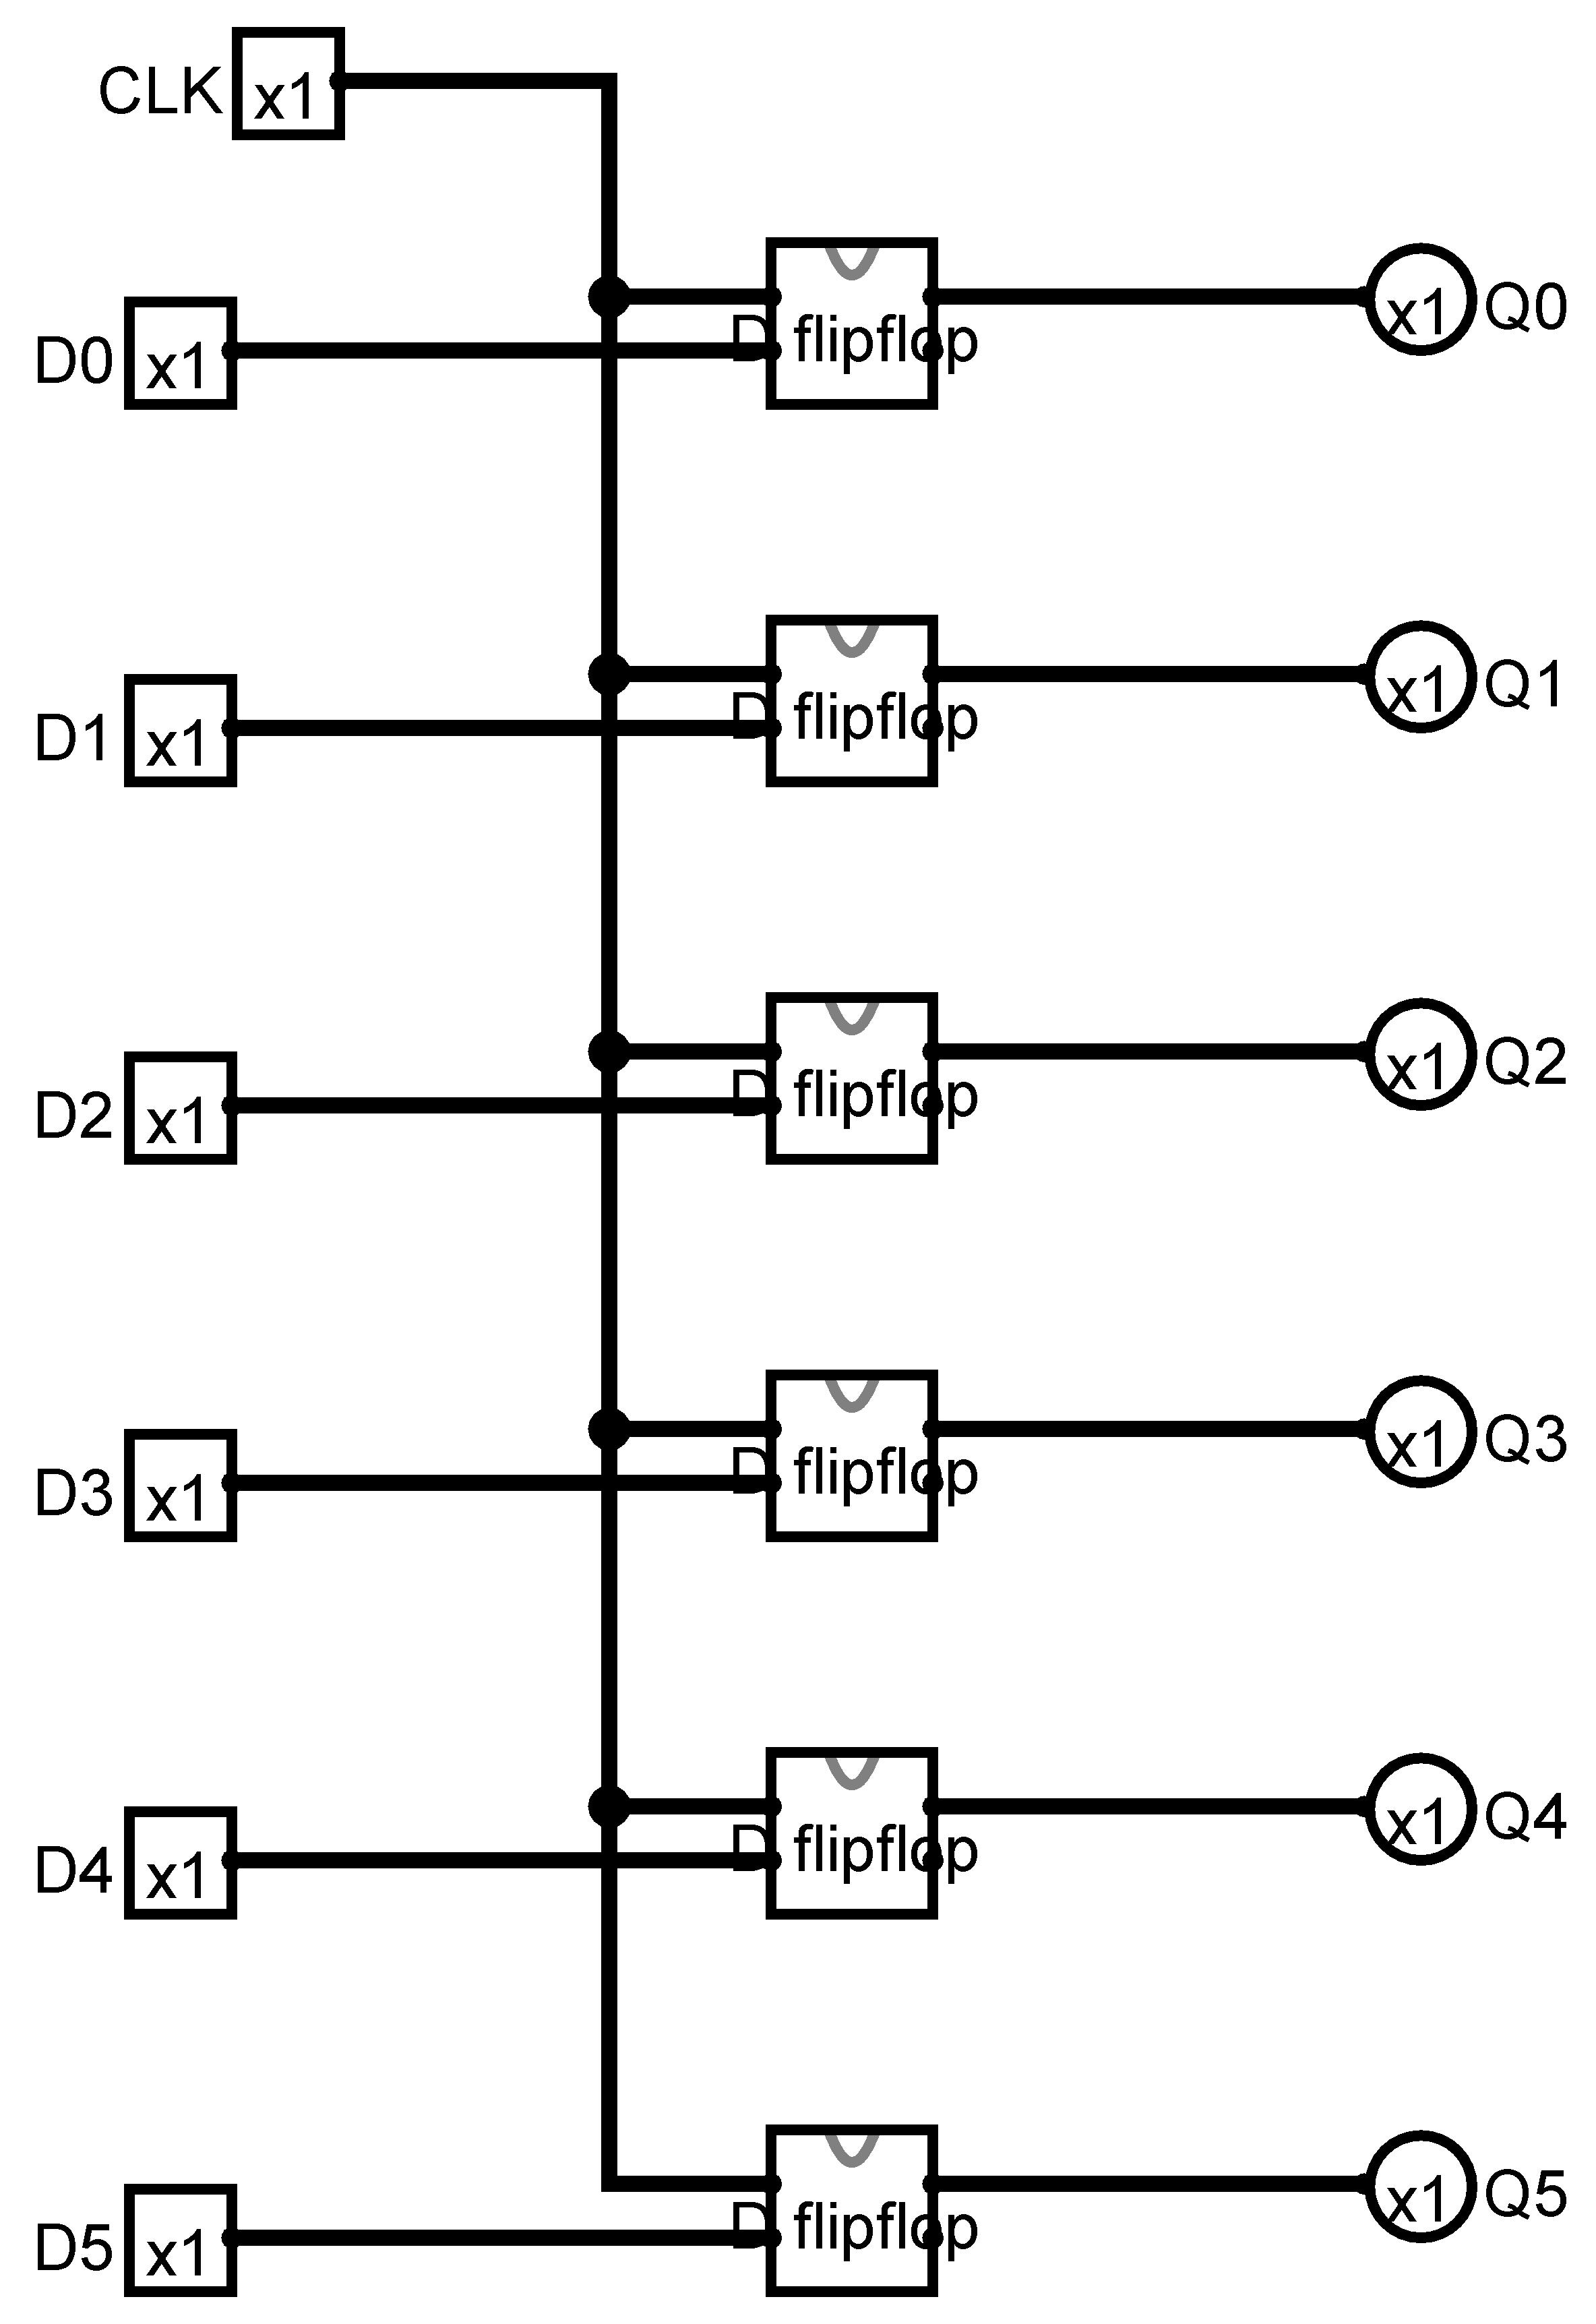
\includegraphics[width=0.4\textwidth]{6-bit Register.jpg}
    \caption{Circuito digital de un registro de 6 bits.}
    \label{fig:6bitRegister}
\end{figure}

El registro puede guardar distintos estados en un solo bloque de circuito, y los recuerda mientras no llegue el \textit{Clock edge}.
Una vez terminados los registros, podemos empezar esta tarea.

Se nos pide que, utilizando una seria de registros y un contador simple, emulemos los distintos escenarios de enfrentamientos del ExaBot, por lo que para esto, debimos modificar un poco el circuito original, donde implementamos un \textit{restador de 1 bit}, que mantenia una cuenta de la batería del ExaBot, y se uso un multiplexor para distinguir entre el primer escenario y el resto. El resto de cambios son visibles en la imagen:
\newpage

\begin{figure}[!htbp]
    \centering
    \includegraphics[width=0.95\textwidth]{Circuito combi.jpg}
    \caption{Circuito combinacional del movimiento del ExaBot, con ajustes para su funcionamiento secuencial}
    \label{fig:CircCombiNuevo}
\end{figure}

Una vez realizados los ajustes al circuito combinacional, podemos empezar a armar el circuito secuencial, basado en una \textit{FSM}, este circuito consiste en 15 registros, que son actualizados por un clock, y que entregan la informacion a cada circuito, y además, cada circuito entrega informacion de la batería al circuito que le es siguiente, lo que permite que sea secuencial.

A continuación se puede observar en la siguiente imagen el resultado de modelar el circuito en el software \textit{Logisim}:

\newpage


\begin{figure}[!htbp]
    \centering
    \includegraphics[width=1\textwidth]{main1.jpg}
    \caption{Circuito secuencial: Primer, segundo y tercer registro y CC.}
    \label{fig:CircSec1}
\end{figure}

\newpage


\begin{figure}[!htbp]
    \centering
    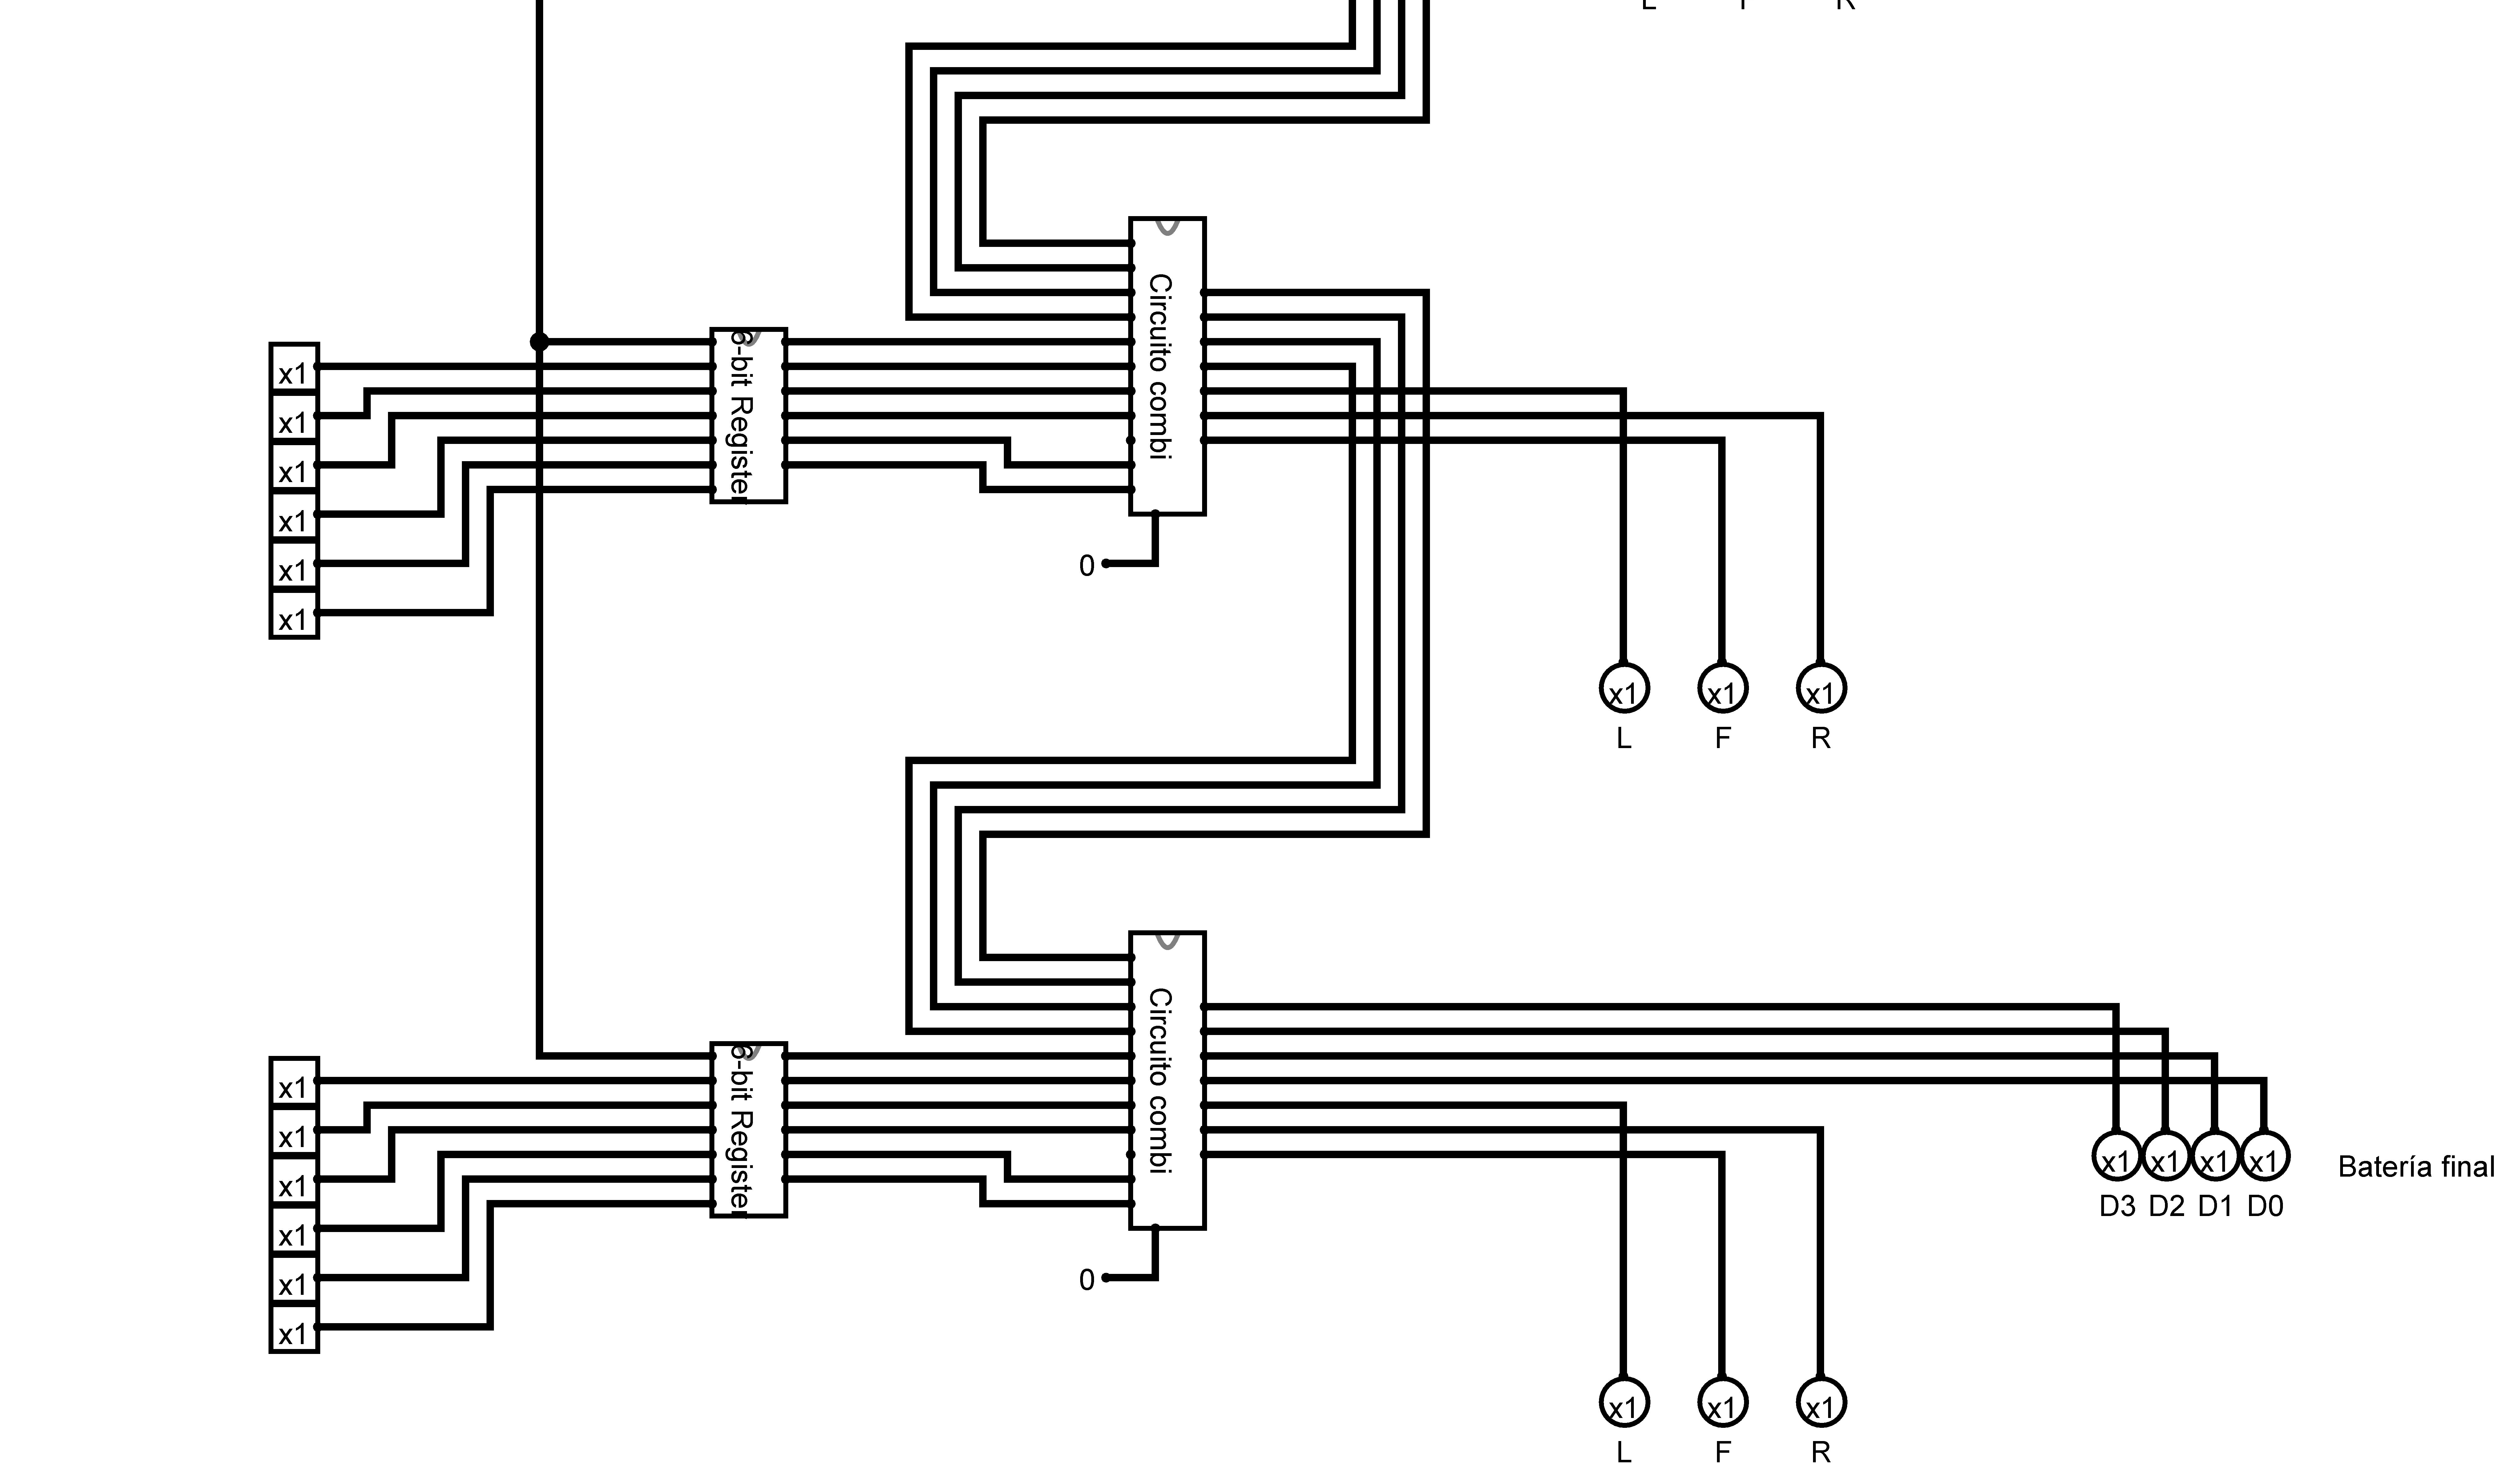
\includegraphics[width=1\textwidth]{main2.jpg}
    \caption{Circuito secuencial: registro y CC número 14 y 15.}
    \label{fig:CircSec2}
\end{figure}

Nótese que en las imágenes solo se muestran los registros 1, 2, 3, 14 y 15, puesto que la imagen es muy grande, pero todos los registros que no son mostrados, son iguales a los registros 2, 3 y 14.

Y mediante este proceso de construccion de los bloques de circuito digital necesario, pudimos construir un circuito secuencial que funciona, y esto último lo revisaremos en la siguiente sección de este informe.

\section{Resultados y análisis}
Al ser tan grandes las imágenes del circuito completo, no es feasible mostrarlas o incorporarlas al informe, pero serán agregadas a la carpeta de entrega de esta tarea.

Se puede analizar que el circuito cumple su función y va restando batería por cada iteracion y recargando esta en cada caso que corresponde.


\section{Conclusiones}
Y así es como mediente un proceso de construccion modularizada y análisis de circuitos, logramos construir un circuito secuencial que cumple la funcion pedida y consigue afectar el resultado de las siguientes iteraciones del mismo. 


\end{document}
